\providecommand{\main}{../..}
\documentclass[\main/thesis.tex]{subfiles}
\begin{document}

\section{Continuous Systems [work in process]}\label{continuous}

We say a numeral system is \textit{continuous} if there are no gaps in the number
line and we can always find a successor after each numeral.
In other words, a system is continuous if every numeral is \textit{incrementable}.

\begin{lstlisting}
Continuous : ∀ b d o → Set
Continuous b d o = (xs : Numeral b d o) → Incrementable xs
\end{lstlisting}

Bounded systems are deemed to be incontinuous because there are no successor
after the maximum numeral.

\begin{lstlisting}
Bounded⇒¬Continuous : ∀ {b d o}
    → Bounded b d o
    → ¬ (Continuous b d o)
Bounded⇒¬Continuous (xs , max) claim
    = contradiction (claim xs) (Maximum⇒¬Incrementable xs max)
\end{lstlisting}

Since systems of \lstinline|NullBase| and \lstinline|AllZeros| are all bounded,
they cannot be continuous. We will only be concerning ourselves with systems of
\lstinline|Proper| in the rest of the section.

Suppose we want to determine if a system of \lstinline|Proper| is continuous,
we can examine \textit{every} numeral of that system with the view function
\lstinline|nextView|.
If \textit{all} numerals are sorted as \lstinline|Interval| and
\lstinline|UngappedEndpoint|, then the system is continuous;
if \textit{any} numeral is sorted as \lstinline|GappedEndpoint|,
then the system must not be continuous.

But it is impossible to go through every numeral because we know that systems
of \lstinline|Proper| are non-exhaustive.
Therefore we need another way of deciding the continuity of a system.

\subsection{Look no further than the Gaps}

In the section~\ref{next}, we have propositions for describing gaps.

\begin{lstlisting}
Gapped#0 : ∀ b d o → Set
Gapped#0 b d o = suc d < carry o * suc b

Gapped#N : ∀ b d o
    → (xs : Numeral (suc b) (suc d) o)
    → (proper : 2 ≤ suc (d + o))
    → Set
Gapped#N b d o xs proper
    = suc d < (⟦ next-numeral-Proper xs proper ⟧ ∸ ⟦ xs ⟧) * suc b

Gapped : ∀ {b d o}
    → (xs : Numeral (suc b) (suc d) o)
    → (proper : 2 ≤ suc (d + o))
    → Set
Gapped {b} {d} {o} (x ∙)    proper = Gapped#0 b d o
Gapped {b} {d} {o} (x ∷ xs) proper = Gapped#N b d o xs proper
\end{lstlisting}

\lstinline|Gapped#0| describes the first gap of a system, whereas
\lstinline|Gapped#N| covers the rest.
Compared to \lstinline|Gapped#N|, the definition of \lstinline|Gapped#0| is much
less demanding because it only depends on the three indices, making it really
easy to be determined.

\subsection{When the First Gap is Open}

Let's start with the easier case, we can know for sure that when the first gap
\lstinline|Gapped#0| is open, the system must not be continuous.

\begin{center}
    \begin{adjustbox}{max width=\textwidth}
        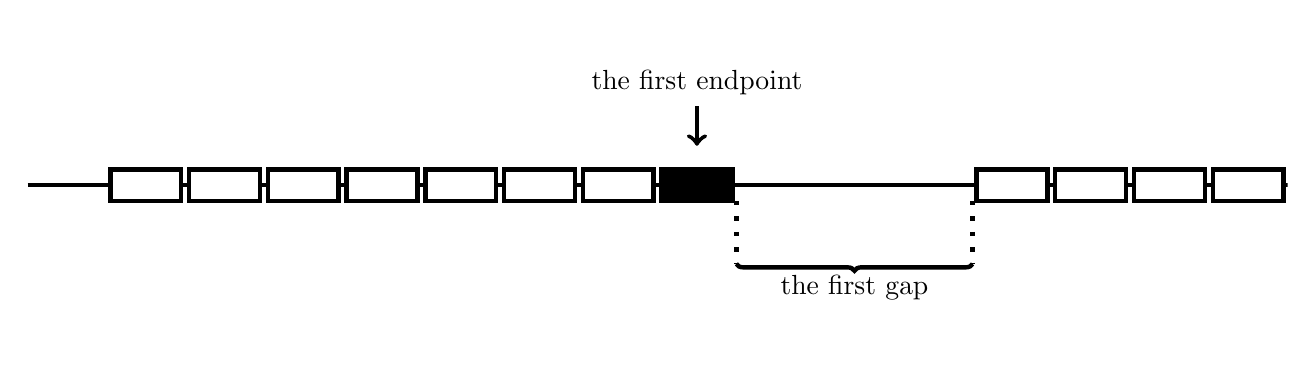
\begin{tikzpicture}
            % the frame
            \path[clip] (0, -2) rectangle (16, 2);
            % the spine
            \draw[ultra thick] (0,0) -- (16,0);
            % the body

            \foreach \i in {1,...,7} {
                \draw[ultra thick, fill=white] ({\i+0.05}, -0.2) rectangle ({\i+0.95}, +0.2);
            };
            \draw[ultra thick, fill=black] (8.05, -0.2) rectangle (8.95, +0.2);

            \foreach \i in {12,...,16} {
                \draw[ultra thick, fill=white] ({\i+0.05}, -0.2) rectangle ({\i+0.95}, +0.2);
            };
            \draw[->, ultra thick] (8.5,1) -- (8.5,0.5)
                node at (8.5, 1.3) {the first endpoint};

            % gap
            \draw[ultra thick, loosely dotted] (9, -0.2) -- (9,-1);
            \draw[ultra thick, loosely dotted] (12,-0.2) -- (12,-1);
            \draw[ultra thick, decoration={brace,mirror},decorate]
                (9, -1) -- (12,-1);
            \node at (10.5, -1.3) {the first gap};
        \end{tikzpicture}
    \end{adjustbox}
\end{center}

We construct the first endpoint with the greatest digit.

\begin{lstlisting}
first-endpoint : ∀ b d o → Numeral (suc b) (suc d) o
first-endpoint b d o = greatest-digit d ∙
\end{lstlisting}

The first endpoint is proven to be not incrementable.

\begin{lstlisting}
first-endpoint-¬Incrementable : ∀ {b d o}
    → (proper : 2 ≤ suc (d + o))
    → (gapped : Gapped#0 b d o)
    → ¬ (Incrementable (first-endpoint b d o))
first-endpoint-¬Incrementable {b} {d} {o} proper gapped
    with nextView (first-endpoint b d o) proper
first-endpoint-¬Incrementable proper gapped
    | Interval b d o ¬greatest
    = contradiction (greatest-digit-is-the-Greatest d) ¬greatest
first-endpoint-¬Incrementable proper gapped
    | GappedEndpoint b d o greatest _
    = GappedEndpoint⇒¬Incrementable
        (first-endpoint b d o) greatest proper gapped
first-endpoint-¬Incrementable proper gapped
    | UngappedEndpoint b d o greatest ¬gapped
    = contradiction gapped ¬gapped
\end{lstlisting}

The first endpoint can then be used as an counter example of the continuity of
the system.

\begin{lstlisting}
Gapped#0⇒¬Continuous : ∀ {b d o}
    → (proper : 2 ≤ suc (d + o))
    → (gapped : Gapped#0 b d o)
    → ¬ (Continuous (suc b) (suc d) o)
Gapped#0⇒¬Continuous {b} {d} {o} proper gapped cont
    = contradiction
        (cont (first-endpoint b d o))
        (first-endpoint-¬Incrementable proper gapped)
\end{lstlisting}

Now we can see if a system is incontiuous just by checking the first gap.

\begin{lstlisting}
Continuous-Proper : ∀ b d o
    → (proper : 2 ≤ suc (d + o))
    → Dec (Continuous (suc b) (suc d) o)
Continuous-Proper b d o proper with Gapped#0? b d o
Continuous-Proper b d o proper | yes gapped#0
    = no (Gapped#0⇒¬Continuous proper gapped#0)
Continuous-Proper b d o proper | no ¬gapped#0
    = ?
\end{lstlisting}

However, when the first gap is closed, it is uncertain whether the given system
will be continuous.

\subsection{When the First Gap is Closed}

If we can prove that \lstinline|Gapped#N| \textbf{implies} \lstinline|Gapped#0|,
then by contraposition, we can know that all gap of a system are closed if the
first gap is also closed.

\begin{lstlisting}[basicstyle=\ttfamily\scriptsize]
Gapped#N⇒Gapped#0 : ∀ {b d o}
    → (xs : Numeral (suc b) (suc d) o)
    → (proper : 2 ≤ suc (d + o))
    → Gapped#N b d o xs proper
    → Gapped#0 b d o
Gapped#N⇒Gapped#0 xs proper gapped#N with nextView xs proper
Gapped#N⇒Gapped#0 xs proper gapped#N | Interval b d o ¬greatest =
    start
        suc (suc d)
    ≤⟨ gapped#N ⟩
        (⟦ next-numeral-Proper-Interval xs ¬greatest proper ⟧ ∸ ⟦ xs ⟧) * suc b
    ≤⟨ *n-mono (suc b) (...next-numeral-Proper-Interval-lemma xs ¬greatest...) ⟩
        (suc zero ⊔ o) * suc b
    □)
Gapped#N⇒Gapped#0 (x ∙)    proper _ | GappedEndpoint b d o greatest gapped#0
    = gapped#0
Gapped#N⇒Gapped#0 (x ∷ xs) proper _ | GappedEndpoint b d o greatest gapped#N
    = Gapped#N⇒Gapped#0 xs proper gapped#N
Gapped#N⇒Gapped#0 xs proper gapped#N | UngappedEndpoint b d o greatest ¬gapped =
    start
        suc (suc d)
    ≤⟨ gapped#N ⟩
        (⟦ next-numeral-Proper-UngappedEndpoint xs greatest proper ¬gapped ⟧
            ∸ ⟦ xs ⟧) * suc b
    ≤⟨ *n-mono (suc b) (... next-numeral-Proper-UngappedEndpoint-lemma ...) ⟩
        (suc zero ⊔ o) * suc b
    □)
\end{lstlisting}

Here is the contrapositive version of the theorem above.

\begin{lstlisting}
¬Gapped#0⇒¬Gapped#N : ∀ {b d o}
    → (xs : Numeral (suc b) (suc d) o)
    → (proper : 2 ≤ suc (d + o))
    → ¬ (Gapped#0 b d o)
    → ¬ (Gapped#N b d o xs proper)
¬Gapped#0⇒¬Gapped#N xs proper ¬Gapped#0
    = contraposition (Gapped#N⇒Gapped#0 xs proper) ¬Gapped#0
\end{lstlisting}

We can conclude that if the first gap is closed,
then so do the rest of the gaps,
hence the system is continuous.

\begin{lstlisting}[basicstyle=\ttfamily\scriptsize]
¬Gapped#0⇒Continuous : ∀ {b d o}
    → (proper : 2 ≤ suc (d + o))
    → (¬gapped : ¬ (Gapped#0 b d o))
    → Continuous (suc b) (suc d) o
¬Gapped#0⇒Continuous proper ¬gapped xs with nextView xs proper
¬Gapped#0⇒Continuous proper ¬gapped xs | Interval _ _ _ _
    = (next-numeral-Proper xs proper) , ...
¬Gapped#0⇒Continuous proper ¬gapped (x ∙) | GappedEndpoint _ _ _ _ gapped
    = contradiction gapped ¬gapped
¬Gapped#0⇒Continuous proper ¬gapped (x ∷ xs) | GappedEndpoint _ _ _ _ gapped
    = contradiction gapped (¬Gapped#0⇒¬Gapped#N xs proper ¬gapped)
¬Gapped#0⇒Continuous proper _ xs | UngappedEndpoint _ _ _ _ ¬gapped
    = (next-numeral-Proper xs proper) , ...
\end{lstlisting}

\subsection{Determining Continuity}

Finally, we can decide if a system is continuous.

\begin{lstlisting}[basicstyle=\ttfamily\scriptsize]
Continuous-Proper : ∀ b d o
    → (proper : 2 ≤ suc (d + o))
    → Dec (Continuous (suc b) (suc d) o)
Continuous-Proper b d o proper with Gapped#0? b d o
Continuous-Proper b d o proper | yes gapped#0
    = no (Gapped#0⇒¬Continuous proper gapped#0)
Continuous-Proper b d o proper | no ¬gapped#0
    = yes (¬Gapped#0⇒Continuous proper ¬gapped#0)

Continuous? : ∀ b d o → Dec (Continuous b d o)
Continuous? b d o with numView b d o
Continuous? _ _ _ | NullBase d o = no (Bounded⇒¬Continuous (Bounded-NullBase d o))
Continuous? _ _ _ | NoDigits b o = yes (λ xs → NoDigits-explode xs)
Continuous? _ _ _ | AllZeros b = no (Bounded⇒¬Continuous (Bounded-AllZeros b))
Continuous? _ _ _ | Proper b d o proper = Continuous-Proper b d o proper
\end{lstlisting}

% \subsection{Observations}
%
% \lstinline|Numeral 4 3 0| is a quaternary (base-4) system with only 3 digits:
% $0, 1, 2$.
% Suppose we plot all values of numerals of \lstinline|Numeral 4 3 0| onto a number
% line, it would have a series of gaps that are ever widening as shown in the figure below.
%
% \begin{center}
%     \begin{adjustbox}{max width=\textwidth}
%         \begin{tikzpicture}[spy using outlines]
%
%             \foreach \j in {0,...,2} {
%                 \foreach \i in {0,...,2} {
%                     \draw[fill=black] ({\j*4 + \i}, 0.5) rectangle ({\j*4 + \i + 0.75}, 0.75);
%                 };
%             };
%
%             \draw[ultra thick] (0, 0) -- (16, 0);
%
%             % ticks
%             \foreach \i in {0, ..., 64} {
%                 \draw[thick] ({\i*0.25},0) -- ({\i*0.25},-0.2);
%             };
%             \foreach \i in {0, ..., 16} {
%                 \pgfmathsetmacro{\j}{int(\i * 4)}
%                 \draw[thick] (\i,0) -- (\i,-0.3)
%                     node[below, scale=0.8] {\j};
%             };
%
%             % spies
%             \spy[rectangle,lens={scale=8}, size=5cm, connect spies]
%                 on (0.875,0.75) in node [left] at (5.25,5);
%             \spy[rectangle,lens={scale=2}, size=5cm, connect spies]
%                 on (3.375,0.75) in node [left] at (10.5,5);
%
%             % gaps
%             \draw[ultra thick, loosely dotted] (1.75,5) -- (1.75,6);
%             \draw[ultra thick, loosely dotted] (3.75,5) -- (3.75,6);
%             \draw[ultra thick, decoration={brace,mirror},decorate]
%                 (3.75, 6) -- (1.75, 6);
%             \node at (2.75, 6.5) {$1$};
%             \draw[ultra thick, loosely dotted] (6.75,5) -- (6.75,6);
%             \draw[ultra thick, loosely dotted] (9.25,5) -- (9.25,6);
%             \draw[ultra thick, decoration={brace,mirror},decorate]
%                 (9.25, 6) -- (6.75,6);
%             \node at (8, 6.5) {$5$};
%             \draw[ultra thick, loosely dotted] (10.75, 0.5) -- (10.75,6);
%             \draw[ultra thick, loosely dotted] (16,0.5) -- (16,6);
%             \draw[ultra thick, decoration={brace,mirror},decorate]
%                 (16, 6) -- (10.75,6);
%             \node at (13.375, 6.5) {$21$};
%
%         \end{tikzpicture}
%     \end{adjustbox}
% \end{center}
%
% \subsection{The Relation between Gaps}
%
% In the section~\ref{next}, we have propositions for describing these gaps.
%
% \begin{lstlisting}
% Gapped#0 : ∀ b d o → Set
% Gapped#0 b d o = suc d < carry o * suc b
%
% Gapped#N : ∀ b d o
%     → (xs : Numeral (suc b) (suc d) o)
%     → (proper : 2 ≤ suc (d + o))
%     → Set
% Gapped#N b d o xs proper
%     = suc d < (⟦ next-numeral-Proper xs proper ⟧ ∸ ⟦ xs ⟧) * suc b
%
% Gapped : ∀ {b d o}
%     → (xs : Numeral (suc b) (suc d) o)
%     → (proper : 2 ≤ suc (d + o))
%     → Set
% Gapped {b} {d} {o} (x ∙)    proper = Gapped#0 b d o
% Gapped {b} {d} {o} (x ∷ xs) proper = Gapped#N b d o xs proper
% \end{lstlisting}
%
% \lstinline|Gapped#0| only describes the first gap of a system, whereas the rest
% of the gaps are covered by \lstinline|Gapped#N|.
% Compared to \lstinline|Gapped#N|, the definition of \lstinline|Gapped#0| is much
% less demanding because it only depends on the three indices, making it really
% easy to be determined.


\end{document}
